\documentclass{beamer}

\usecolortheme[light]{solarized}

\beamertemplatenavigationsymbolsempty

\usepackage{graphicx}
\usepackage{hyperref}
\usepackage{colortbl, xcolor}
\usepackage{booktabs}

\usepackage{tikz}
\usetikzlibrary{calc}

\title{Fellowship plans}
\author{@drvinceknight}
\date{2016-02-03}

\begin{document}

\frame{\titlepage}

\begin{frame}
    \begin{center}
        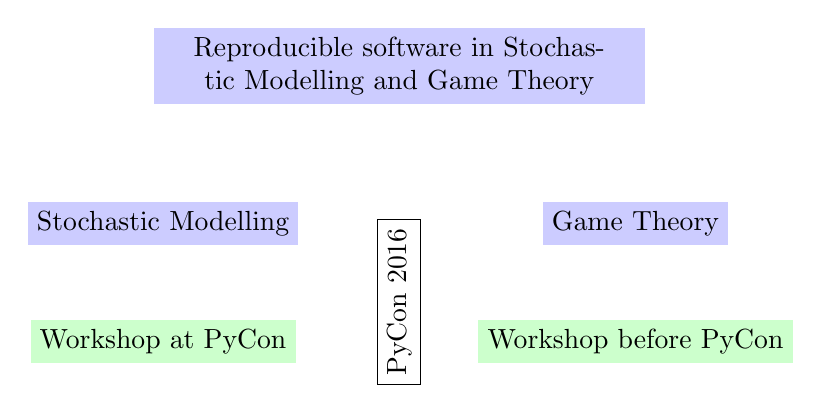
\begin{tikzpicture}
            \node (title) at (0,0) [fill=blue!20, text width = 6cm, align=center]
            {Reproducible software in Stochastic Modelling and Game Theory};
            \node (StochasticModelling) at ($(title) + (-3, -2)$) [fill=blue!20]
            {Stochastic Modelling};

            \node (PyCon) at ($(StochasticModelling) + (0, -1.5)$) [fill=green!20]
            {Workshop at PyCon};

            %-----------------

            \node (GameTheory) at ($(title) + (3, -2)$) [fill=blue!20] {Game Theory};

            \node (gt) at ($(GameTheory) + (0, -1.5)$) [fill=green!20]
            {Workshop before PyCon};

            {Game Theory};

            \node (PyConuk) at (0, -3) [rotate=90, draw] {PyCon 2016};
        \end{tikzpicture}
    \end{center}
\end{frame}

\begin{frame}
    \begin{center}
        \begin{tabular}{cc|c}
            \toprule
            Wednesday                 & Thursday     & Friday (PyConUK)\\
            \midrule
            \cellcolor{blue!20} GT Talks & \cellcolor{blue!20} GT Workshops &
            \cellcolor{yellow!20}Stochastic workshop\\
            \bottomrule
        \end{tabular}
    \end{center}
\end{frame}

\begin{frame}
    \begin{center}
        \huge Computational Game Theory
    \end{center}
    \begin{center}
        Topics
    \end{center}
    \begin{itemize}
        \item Gambit
        \item Game theory in Sagemath
        \item Iterated Prisoner's Dilemma (axelrod package)
    \end{itemize}
    \pause
    \begin{center}
        Todo
    \end{center}
    \begin{itemize}
        \item Funding
        \item Speakers
    \end{itemize}
\end{frame}

\begin{frame}
    \begin{center}
        \huge Stochastic workshop
    \end{center}
\end{frame}

\end{document}
